\section{Deterministic Finite Automata (DFA)}
A DFA is a 5-tuple $A = (Q, \Sigma, \delta, q_0, F)$ where:
\begin{description}
    \item[$Q:$] finite (non-empty) set of states;
    \item[$\Sigma:$] alphabet of input symbols;
    \item[$\delta:$] transition function:
        $$
            \delta: Q \times \Sigma \to Q
        $$
    \item[$q_0:$] start state:
        $$
            q_0 \in Q
        $$
    \item[$F:$] set of final states:
        $$
            F \subseteq Q
        $$
\end{description}

\subsection{Transition Table}
Transitional Table is a tabular representation of this transition function.

\subsection{Transition Diagram}
Transitional Diagram is a graph where:
\begin{itemize}
    \item for each state in the automaton there a node;
    \item for each transition $\delta(p, a) = q$ there is an arc from $p$ to $q$ labelled $a$.
\end{itemize}
The start state has an entering non-labelled arc and the final states are marked by a double circle.

\section{Non-Deterministic Finite Automata (NFA)}
An NFA is a 5-tuple $A = (Q, \Sigma, \delta, q_0, F)$ where:
\begin{description}
    \item[$Q:$] finite (non-empty) set of states;
    \item[$\Sigma:$] alphabet of input symbols;
    \item[$\delta:$] transition function:
        $$
            \delta: Q \times \Sigma \to \mathscr{P}(Q)
        $$
        $\mathscr{P}(Q)$: powerset of Q (the set of all subsets)
        $$
            \|\mathscr{P}(Q)\| = 2^{\|Q\|}
        $$
    \item[$q_0:$] start state:
        $$
            q_0 \in Q
        $$
    \item[$F:$] set of final states:
        $$
            F \subseteq Q
        $$
\end{description}
NB: a DFA is a special case of NFA.

\section{Equivalence of NFA and DFA}
\begin{figure}[H]
    \centerline{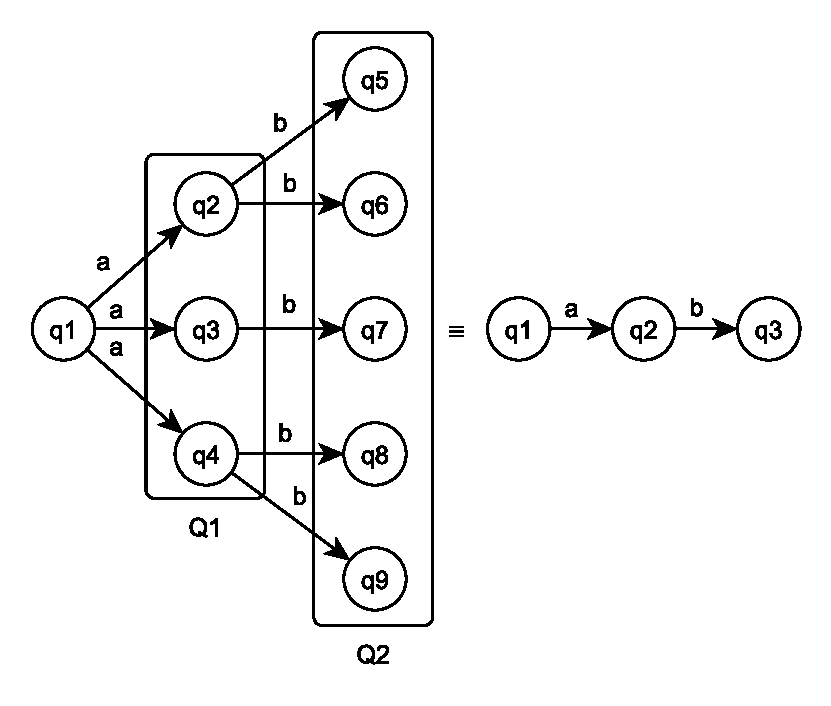
\includegraphics[width=0.6\textwidth]{img/1.pdf}}
\end{figure}
\begin{align*}
    Q_1 &= \left\{q_2, q_3, q_4\right\}\\
    Q_2 &= \left\{q_5, q_6, q_7, q_8, q_9\right\}
\end{align*}

Let $N = (Q_n, \Sigma, \delta_n, q_0, F_n)$ be an NFA; let us construct a DFA $D = (Q_d, \Sigma, \delta_d, \left\{q_0\right\}, F_d)$ where:
\begin{itemize}
    \item $Q_d \subseteq \mathscr{P}(Q_n)$;
    \item $\delta_d(S, a) = \cup_i \delta_n(p_1, a)$ where $p_i \in S \in Q_d$;
    \item $F_d = \left\{S \middle| S \in Q_d; S \cap F_n \neq \emptyset \right\}$.
\end{itemize}
By construction $L(D) = L(N)$, so $NFA \equiv DFA$

\section{From Finite Automata to Regular Expression}
It is possible to eliminate states in a Finite Automata by maintaining all the paths and by labelling the transitions with regular expressions:
\begin{figure}[H]
    \centerline{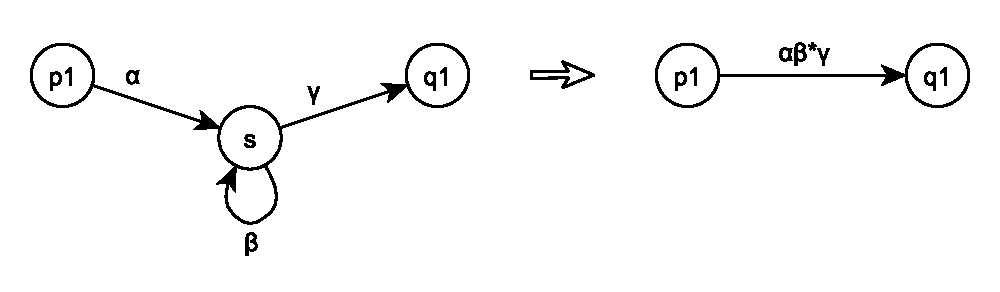
\includegraphics[width=0.7\textwidth]{img/2.pdf}}
\end{figure}
Given a finite state automaton $FA = (Q, \Sigma, \delta, q_0, F)$, add an initial state $A$ and a final state $\Omega$:
\begin{figure}[H]
    \centerline{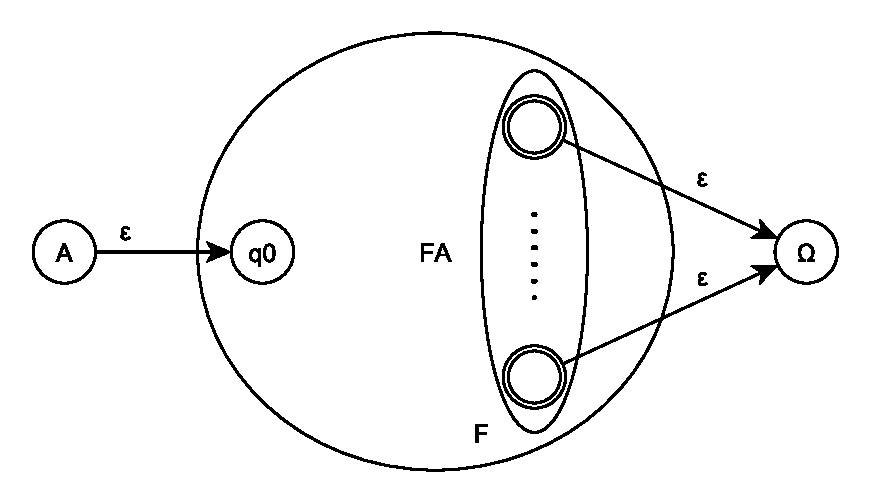
\includegraphics[width=0.7\textwidth]{img/3.pdf}}
\end{figure}
\begin{itemize}
    \item eliminate all the states in $FA$;
    \item the union of the labels on the transitions from $A$ to $\Omega$ gives the regular expression of the language $L(FA)$.
\end{itemize}

\section{From Regular Expression to Finite Automata}

\subsection{Regular Sets}
The regular sets: $0$, $\left\{\varepsilon\right\}$, $\left\{a\right\}$, $a \in \Sigma$ are accepted by finite state automata.
\begin{figure}[H]
    \centerline{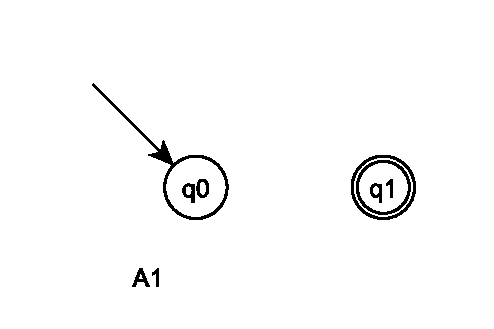
\includegraphics[width=0.4\textwidth]{img/4.pdf}}
\end{figure}
$$
    L(A_1) = 0
$$
\begin{figure}[H]
    \centerline{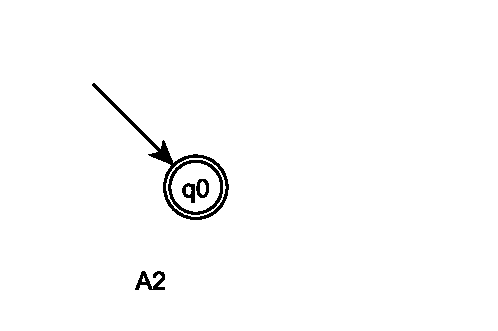
\includegraphics[width=0.4\textwidth]{img/5.pdf}}
\end{figure}
$$
    L(A_2) = \left\{\varepsilon\right\}
$$
\begin{figure}[H]
    \centerline{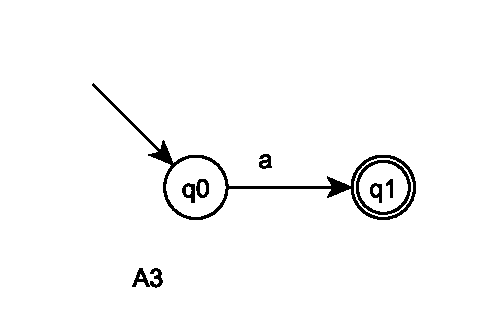
\includegraphics[width=0.4\textwidth]{img/6.pdf}}
\end{figure}
$$
    L(A_3) = \left\{a\right\}, a \in \Sigma
$$
Let $A_1 = (Q_1, \Sigma, \delta_1, q_{01}, F_1)$ and $A = (Q_2, \Sigma, \delta_2, q_{02}, F_2)$ be finite state automata; the language $L(A_1) \cup L(A_2)$ is accepted by a finite state automaton $A_4$:
\begin{figure}[H]
    \centerline{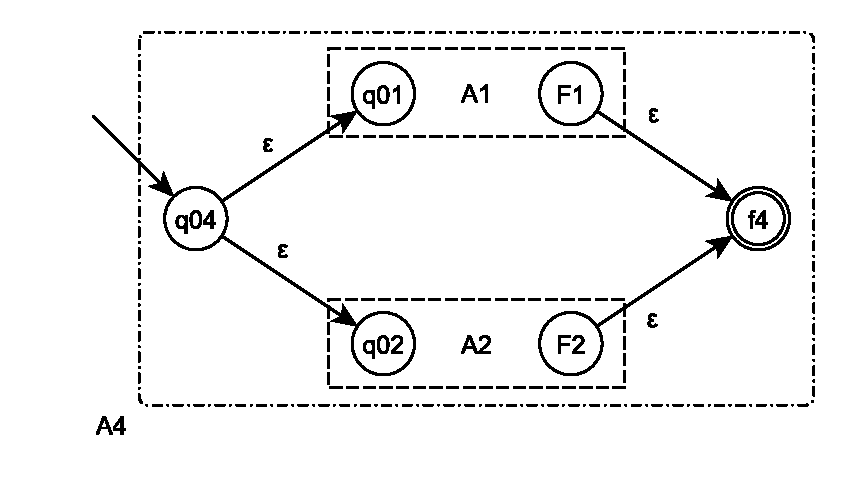
\includegraphics[width=0.7\textwidth]{img/7.pdf}}
\end{figure}

The language $L(A_1)L(A_2)$ is accepted by a finite state automaton $A_5$:
\begin{figure}[H]
    \centerline{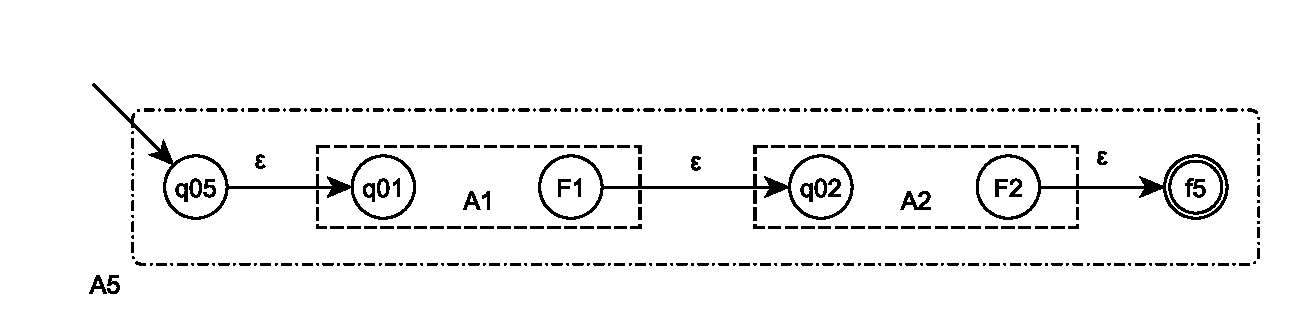
\includegraphics[width=1\textwidth]{img/8.pdf}}
\end{figure}

The language $L(A_1)^\ast$ is accepted by a finite state automaton $A_6$:
\begin{figure}[H]
    \centerline{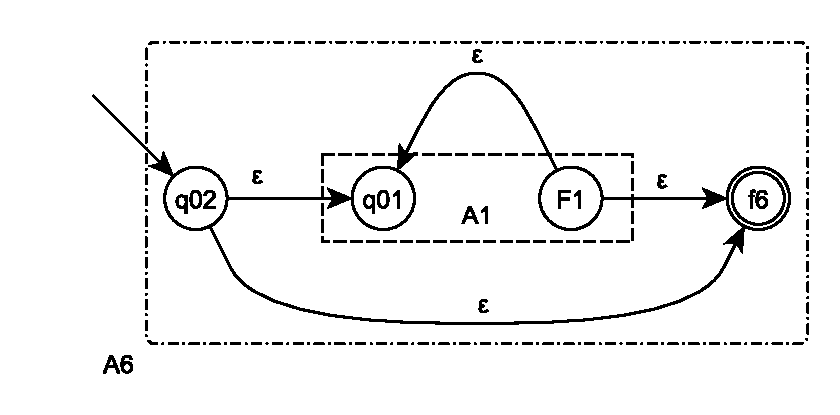
\includegraphics[width=0.7\textwidth]{img/9.pdf}}
\end{figure}

\section{Non-Deterministic Finite State Automata with $\varepsilon\text{-transition}$ ($\varepsilon\text{-NFA}$)}
In the construction of a Finite State Automaton from regular expressions, the $\varepsilon\text{-transitions}$ make the automata \emph{non-deterministic}.
The function $\varepsilon\text{-closure}(q)$ gives the set of states that can be reached (recursively) from state $q$ with empty string.

\subsection{Equivalence of $\varepsilon\text{-NFA}$ and DFA}
Let $N = (Q_n, \Sigma, \delta_n, q_0, F_n)$ be an $\varepsilon\text{-NFA}$; let us construct a DFA $D = (Q_d, \Sigma, \delta_d, \varepsilon\text{-closure}(q_0), F_d)$ where:
\begin{itemize}
    \item $Q_d \subseteq \mathscr{P}(Q_n)$;
    \item $\delta_d(S, a) = \varepsilon\text{-closure}(\cup_i \delta_n(p_i, a))$ where $p_i \in S \in Q_d$;
    \item $F_d \left\{S \middle| S \in Q_d; S \cap F_n \neq \emptyset\right\}$
\end{itemize}
By construction $L(D) = L(N)$.

\section{Finite Automaton $\equiv$ Regular Languages}
\begin{itemize}
    \item Let $G = (N, T, P, S)$ be a \underline{Right-Regular} grammar; let us construct an FA $A = (Q, T, \delta, S, F)$ where:
    \begin{itemize}
        \item $Q = N \cup \left\{\Omega\right\}$ with $\Omega \in N$;
        \item $F = \left\{\Omega\right\}$;
        \item $
            \delta = \begin{Bmatrix}
                \delta(A, a) = B \quad \text{if} \quad A \to aB \in P \\
                \delta(A, a) = \Omega \quad \text{if} \quad A \to a \in P
            \end{Bmatrix}
        $
    \end{itemize}
    By construction $L(G) = L(A)$.
    \item Let $G = (N, T, P, S)$ be a \underline{Left-Regular} grammar; let us construct an FA $A = (Q, T, \delta, I, \left\{S\right\})$ where:
    \begin{itemize}
        \item $Q = N \cup \left\{I\right\} \quad \text{with} \quad I \notin N$;
        \item $F = \left\{S\right\}$;
        \item $
            \delta = \begin{Bmatrix}
                \delta(B, a) = B \quad \text{if} \quad A \to Ba \in P \\
                \delta(I, a) = \Omega \quad \text{if} \quad A \to a \in P
            \end{Bmatrix}
        $
    \end{itemize}
    By construction $L(G) = L(A)$.
\end{itemize}

\section{Minimum-State DFA}
Let $DFA = (Q, \Sigma, \delta, q_0, F)$ be a deterministic finite automaton, then:
\begin{itemize}
    \item two states $p$ and $q$ of DFA are distinguishable if there is a string $w \in \Sigma^\ast$ such that $\delta(p, w) \in F$ and $\delta(q, w) \in F$;
    \item two states $p$ and $q$ of DFA are equivalent ($p \equiv q$) if they are \emph{non-distinguishable} for any string $w \in \Sigma^\ast$.
\end{itemize}
A DFA is \emph{minimum-state} if it does not contain equivalent states.

Two states $p$ and $q$ of a DFA are $m\text{-equivalent}$ ($p \equiv_m q$) if they are non-distinguishable for all strings $w \in \Sigma^\ast$ with $\|w\| \leq m$.
The equivalent states can be determined by partitioning the set $Q$ in classes of $m\text{-equivalent}$ states, for $m = 0, 1, \ldots, \|Q\| - 2$.

\section{Complement of a Regular Language}
The complement of a regular language is a regular language.

Let $DFA = (Q, \Sigma, \delta, q_0, F)$ be a completely specified deterministic finite automaton, that is there is a transition on every symbol of $\Sigma$ from every state.
The automaton $DFA_c = (Q, \Sigma, q_0, Q - F)$ accepts the language
$$
    L(DFA_c) = \Sigma^\ast - L(DFA) = \neg L(DFA)
$$

\section{Intersection of Regular Languages}
The intersection of two regular languages is a regular language.
$$
    L_1 \cap L_2 = \neg (\neg L_1 \cup \neg L_2)
$$
Let $DFA_1 = (Q_1, \Sigma, \delta_1, q_{01}, F_1)$ and $DFA_2 = (Q_2, \Sigma, \delta_2, q_{02}, F_2)$; the automaton $DFA1 = (Q_1 \times Q_2, \Sigma, \delta, (q_{01}, q_{02}), F_1 \times F_2)$ accepts the language
$$
    L(DFA_1) = L(DFA1) \cap L(DFA_2)
$$

\section{Equivalence of Regular Languages}
It is possible to test if two regular languages are the same:
\begin{itemize}
    \item $DFA_1 = (Q_1, \Sigma, \delta_1, q_{01}, F_1)$;
    \item $DFA_2 = (Q_2, \Sigma, \delta_2, q_{02}, F_2)$.
\end{itemize}
Let us find the equivalence states in the set $Q_1 \cup Q_2$:
$$
    \text{if} \quad q_{01} \equiv q_{02} \quad \text{then} \quad L(DFA_1) = L(DFA_2)
$$